% This is the tex file for ISVLSI16 submission
% by Kaiyuan Guo

% \documentclass{sig-alternate-05-2015}
\documentclass[10pt, conference, compsocconf]{IEEEtran}

\usepackage{amsmath,amsfonts,amssymb}
\usepackage{graphicx}
\usepackage{subfigure}
\usepackage{algorithm}
\usepackage{algorithmicx}
\usepackage{algpseudocode}
\usepackage{caption}
\usepackage{multirow}
\usepackage{textcomp,booktabs}
\usepackage[usenames,dvipsnames]{color}
\usepackage{colortbl}
\usepackage{indentfirst}
\usepackage{url}
\usepackage{cite}
\usepackage{bibspacing}
\usepackage{threeparttable}
\usepackage{bigstrut}

\begin{document}

    %\setlength{\baselineskip}{11pt}
    \captionsetup{singlelinecheck=on}

% title
\title{Angel-Eye: A Complete Design Flow for Mapping CNN onto Customized Hardware}

%\author{
%    Kaiyuan Guo$^{1}$, Lingzhi Sui$^{1,2}$, Jiantao Qiu$^{1}$, Song Yao$^{1,2}$, Song Han$^{2,3}$, Yu Wang$^{1}$, Huazhong Yang$^{1}$\\
%    \normalsize{$^{1}$Department of Electronic Engineering, Tsinghua University}\\
%    \normalsize{$^{2}$Deephi Technology Co., Ltd} \hspace{10pt}
%    \normalsize{$^{3}$Stanford University} \\
%    \normalsize{\{gky15@mails.tsinghua.edu.cn, yu-wang@tsinghua.edu.cn\}}
%}
\author{\IEEEauthorblockN{Kaiyuan Guo\IEEEauthorrefmark{1}\IEEEauthorrefmark{2},
Lingzhi Sui\IEEEauthorrefmark{2},
Jiantao Qiu\IEEEauthorrefmark{1},
Song Yao\IEEEauthorrefmark{2} and
Song Han\IEEEauthorrefmark{3}}
\IEEEauthorblockA{\IEEEauthorrefmark{1}Department of Electronic Engineering\\
Tsinghua University,
Beijing, China\\
Email: gky15@mails.tsinghua.edu.cn, yu-wang@tsinghua.edu.cn}
\IEEEauthorblockA{\IEEEauthorrefmark{2}Deephi Technology Co., Ltd, Beijing, China}
\IEEEauthorblockA{\IEEEauthorrefmark{3}Stanford University, Stanford, California, USA}}


\maketitle

%%==============================================================================
%%  Abstract
%%==============================================================================
\begin{abstract}
Convolutional Neural Network (CNN) has become a successful algorithm in the region of artificial intelligence and a strong candidate for many applications. However, for embedded platforms, CNN-based solutions are still too complex to be applied if only CPU is utilized for computation. Various dedicated hardware designs on FPGA and ASIC have been carried out to accelerate CNN, while few of them explore the whole design flow for both fast deployment and high power efficiency. In this paper, we propose Angel-Eye, a programmable and flexible CNN processor architecture, together with compilation tool and runtime environment. Evaluated on Zynq XC7Z045 platform, Angel-Eye is 8$\times$ faster and 7$\times$ better in power efficiency than peer FPGA implementation on the same platform. A demo of face detection on XC7Z020 is also 20$\times$ and 15$\times$ more energy efficient than counterparts on mobile CPU and mobile GPU respectively.
\end{abstract}



%%==============================================================================
%%  Introduction
%%==============================================================================
\section{Introduction} \label{sec:intro}
Convolutional Neural Network (CNN) is one of the state-of-the-art artificial intelligence algorithms. With a large model and enough training data set, CNN generates complex features for certain tasks, which outperforms traditional handcrafted features. Thus CNN can help achieve the top performance in regions like image classification, object detection and even stereo vision. Some audio algorithms also involves CNN as one of the feature extraction steps.

Despite the outstanding performance, CNN is hard to be implemented in daily applications, because of its high computation complexity. Large CNN models can involve up to nearly 40G operations (multiplication or addition) \cite{simonyan2014very} for the inference of one 224$\times$224 image. Larger images in real applications can scale this number up. Thus this kind of applications are usually implemented as a cloud service on large servers. For personal devices, traditional CPU platforms are hardly able to handle CNN models with acceptable processing speed. For tasks like object detection where real-time processing is required, the situation is worse.

GPU offers high degree of parallelization, thus is a good candidate for compute CNN. But usually a batch of images should be processed together to fully utilize the computation capacity. For video processing, this means larger latency for each frame. On the other hand, recent work have shown that the data precision in CNN processing can be reduced from 32-bit floating point to 16-bit fixed point or even less. This means it is possible to achieve better energy efficiency than GPU with customized hardware.

Implementing customized hardware of CNN requires hardware and software co-design. The network should be adjusted to a hardware friendly form. Recent work on CNN have shown that the data format can be compressed from 32-bit floating point to fixed point. This greatly reduces the power and area cost of the hardware. We have shown that 8-bit fixed point is enough for VGG network\cite{simonyan2014very}. Han et al.\cite{han2015learning} compressed the data to 4-bit by weight sharing. Recent work even tries 1-bit weight for classification\cite{Rastegari2016XNOR}.

On the hardware side, an architecture with high efficiency and high flexibility is needed. Zhang et al.\cite{zhang2015optimizing} proposed a floating point accelerator design on FPGA, where the loop unrolling parameter design space is explored for a certain network. But the situation for running different networks are not considered. ASIC design by Du et al.\cite{du2015shidiannao} consumes only 320mW power by a mesh grid design. However, it only supports CNNs with very limited model capacity due to on-chip memory constraint.

Previous work mainly maps the software model to hardware structure manually. But the great variety of the topologies of state-of-the-art CNNs brings challenge to hardware designers. ResNet\cite{he2015deep}, which is the winner of Image-Net Large-Scale Vision Recognition Challenge (ILSVRC) 2016, implements a 152-layer model with shortcut layers. But the winner of 2015 \cite{simonyan2014very} uses cascaded 19 layers in their network.

So a mapping tool is needed to bridge software model with hardware structure. One choice is to automatically generate the hardware code for a certain network. This pushes the hardware performance to the extreme while the flexibility to different networks is low. Another choice is to use a flexible hardware structure and leave the mapping work to software side, which is the choice of our work. This can response to the changes in network topology quickly, no matter the platform is FPGA or ASIC. It also supports different network switch at runtime.

In this paper, we extend our previous work\cite{qiu2016going} to a complete design flow for mapping CNN onto customized hardware. Generally three parts are included in this flow:
\begin{itemize} % \itemsep = 0pt
    \item A data quantization strategy to compress the original network to a fixed-point form.
    \item A parameterized and runtime configurable hardware architecture to support various networks and fit into various platforms.
    \item An instruction set together with a compiler that bridges different topologies of convolutional neural networks with the proposed hardware architecture.
\end{itemize}
Our experiments on FPGA show that the proposed design flow delivers CNN acceleration with high energy efficiency. The rest of this paper is organized as follows. Section \ref{sec:prime} introduces the background of CNN. Related work is then discussed in Section \ref{sec:related_work}. Details of the flow is shown in Section \ref{sec:flow}. We show the experimental results in Section \ref{sec:experiment} and concludes this work in Section \ref{sec:conclusion}.



\section{Preliminary of CNN} \label{sec:prime}
A CNN consists of a set of \emph{layers}. As the name suggests, the most important layers in CNNs are the Conv layers. Besides, FC layers, Non-Linearity layers, and pooling layers (down-sampling layer) are also essential in CNN.

\begin{figure*}[h]
  \centering
  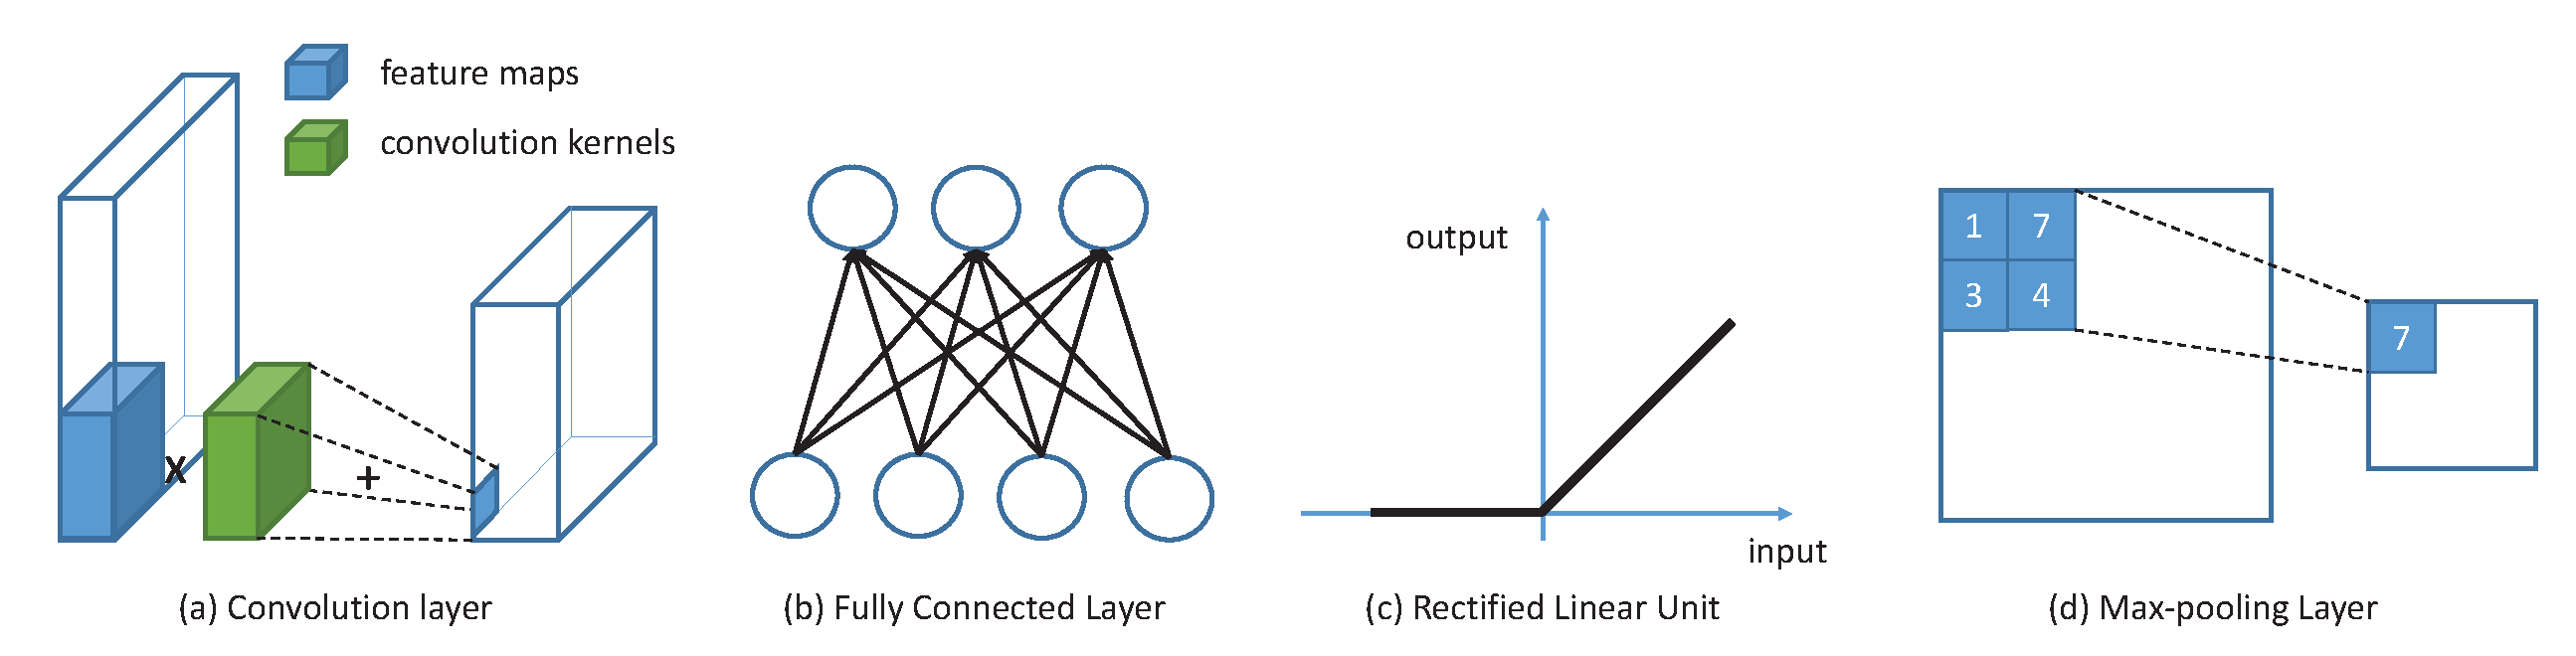
\includegraphics[width=2\columnwidth]{figure/primer.eps}
  \small
  \caption{Typical layers in CNN: (a) Convolutional layer; (b) Fully-Connected layer (dense matrix multiplication); (c) Non-linear layer with Rectified Linear Unit; (d) Max-pooling layer with 2$\times$2 kernel.}
  %\vspace{-10pt}
  \label{fig:primer}
\end{figure*}

\begin{figure*}[h]
  \centering
  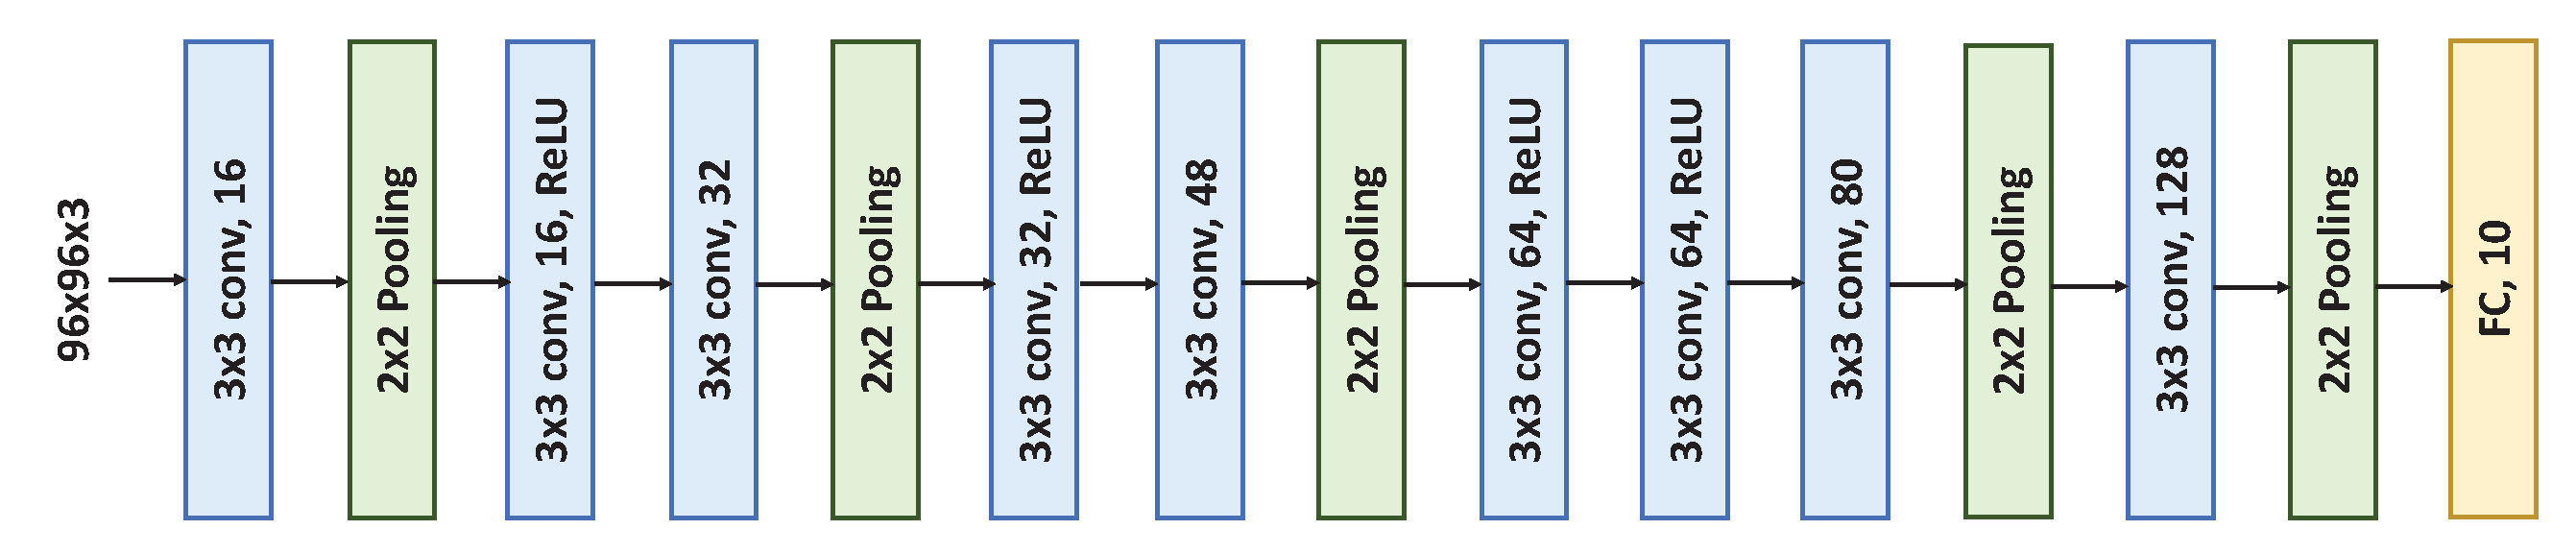
\includegraphics[width=1.8\columnwidth]{figure/alignment_net.eps}
  \small
  %\vspace{-5pt}
  \caption{A practical CNN model for face alignment. For each layer, the kernel size, output channel number and nonlinearity type is given.}
  %\vspace{-10pt}
  \label{fig:face_align_net}
\end{figure*}

\textbf{Conv layer} applies Conv operations on input feature maps and can extract high-level features from the inputs. An example is shown in Figure~\ref{fig:primer} (a), where the feature maps are blue and the 3-D Conv kernel is green. Each pixel of each output feature map is the inner product of a part of input with a 3-D convolution kernel.

\textbf{FC layer} applies a linear transformation on the input feature vector. It is usually used as the classifier in the final stage of a CNN. A simple FC layer is shown in Figure~\ref{fig:primer} (b).

\textbf{Non-linearity layer} helps increase the fitting ability of neural networks. In CNN, the Rectified Linear Unit (ReLU), as shown in Figure~\ref{fig:primer} (c), is the most frequently used function~\cite{krizhevsky2012imagenet}. Hyperbolic tangent function and sigmoid function are also used in various neural networks.

\textbf{Pooling layer} is used for down-sampling. Average pooling and max pooling are two major types of pooling layers. For a pooling layer, it outputs the maximum or average value of each subarea in the input feature map. Pooling layer can not only reduce the feature map size and the computation for later layers, but also introduces translation invariance. A simple max pooling layer with a 2$\times$2 kernel is shown in Figure~\ref{fig:primer} (d).

A practical CNN for face alignment which we use for the verification of our design is shown in Figure~\ref{fig:face_align_net}. It calculates the coordinates of 5 character points of human face given the face image. Conv layers, Pooling layers and Non-linearity layers are interleaved to extract features. An FC layer at the end generates the coordinates of these points from extracted features.

\section{Related Work} \label{sec:related_work}
Though many regions in machine learning benefits from neural network like algorithms, one of the main drawback it brings is the high computation complexity, especially for CNNs. Various accelerator designs for CNN have been proposed. In this section, some state-of-the-art CNNs are introduced first. Then we give an overview of existing CNN accelerators.

\subsection{State-of-the-art CNN}
State-of-the-art CNN models differ greatly from earlier network in topology. Recent work is focusing more on the design of Conv layers than on FC layers. As in VGG network~\cite{simonyan2014very}, 3 FC layers with more than 0.12 billion weights are used for the final classification. ResNet~\cite{he2015deep}, the winner of Image-Net Large-Scale Vision Recognition Challenge (ILSVRC) 2015, implements 152-layers where only the last layer is fully connected. Shortcut structure is also introduced in Conv layers to reinforce the learning ability. Network with no FC layer is also proposed~\cite{long2015fully}.

Convolution kernels in CNN is also changing. Early CNN designs~\cite{krizhevsky2012imagenet}\cite{zeiler2014visualizing} adopted convolution kernels of size 11$\times$11 for Conv layers, which are much larger than the 3$\times$3 kernels in VGG networks~\cite{simonyan2014very} and the 1$\times$1 kernels in SqueezeNet~\cite{iandola2016squeezenet}.  It is a trend to use smaller kernels in Conv Layers. Computation complexity reduces while the network performance remains.

\subsection{CNN Accelerator}
Various architectures have been proposed to accelerate CNN, including both ASIC and FPGA designs. As discussed in~\cite{zhang2015optimizing}, one Conv Layer can be expressed as a 6-layer loop. The key point in CNN accelerator design is the unrolling strategy of the loops for each layer.

Fixed loop unrolling strategy is commonly applied in CNN accelerator designs. Zhang et al.~\cite{zhang2015optimizing} analyzed the data sharing relation of different iterations of a loop to evaluate the cost of unrolling. Calculation on different input channels and that for different output channels are of the lowest cost to be parallelized. But image pixel level and kernel level parallelization are not fully explored. nn-X~\cite{gokhale2014240} adopted 2-D convolver design of size 10$\times$10, which achieves kernel level parallelization. Our previous work~\cite{qiu2016going} uses a 3$\times$3 convolver design targeting at VGG network. ShiDiannao~\cite{du2015shidiannao} implements a mesh grid style structure to achieve parallelization on image pixel level. But the routing cost is rather high. Similar strategy is also adopted by~\cite{sim2016deep}.

Configurable loop unrolling costs much in data routing but can fit into different network topologies better. Chen et al.~\cite{chen2016eyeriss} proposed a 2-D PE array design optimized for CNN. Global bus is used to broadcast and collect data from PEs. The connections are configurable to group different PEs together as convolvers of different sizes. The drawback is the routing cost on extra bits to identify the target PE of the data.


\section{Flow Description}\label{sec:flow}
The overall structure of the design flow is shown in Figure~\ref{fig:flow}. Three parts will be introduced in this section: data quantization, hardware architecture, instruction set and compiler.

\begin{figure}[t]
  \centering
  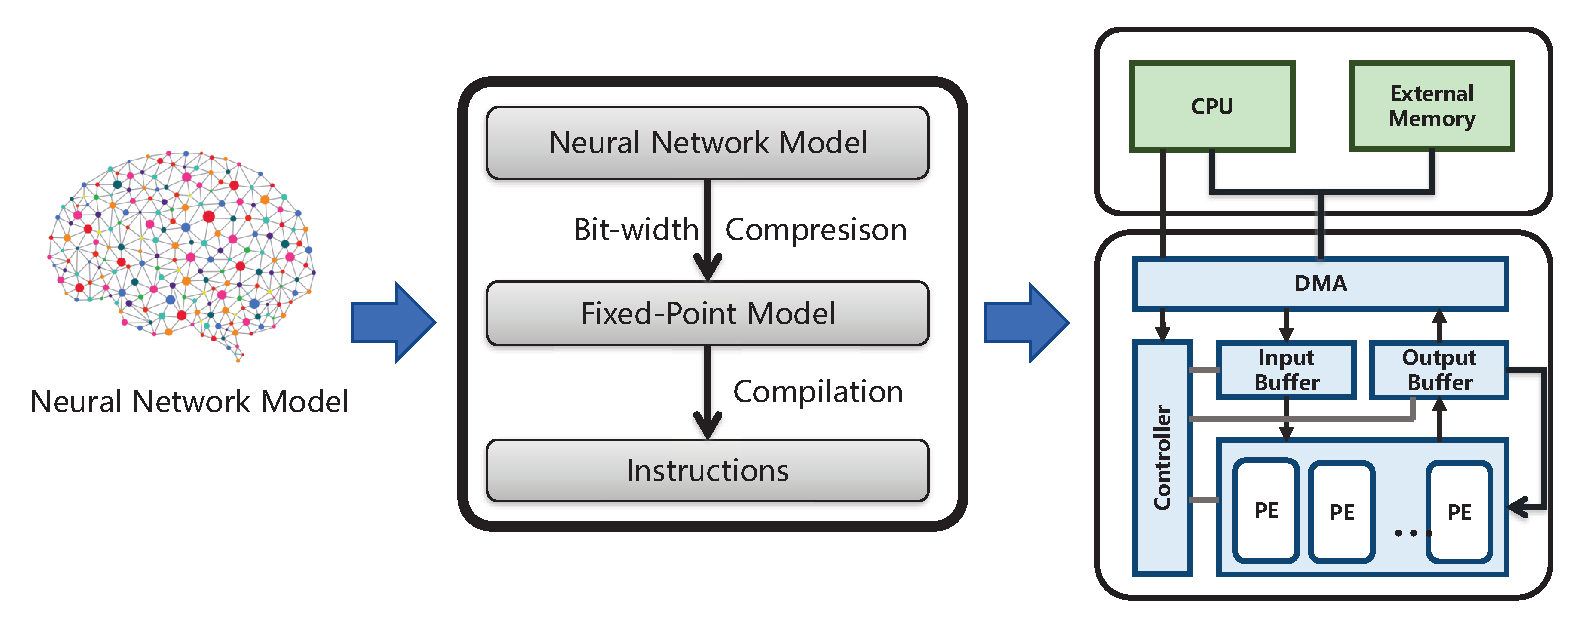
\includegraphics[width=1.0\columnwidth]{figure/figure1.eps}
  \small
  %\vspace{-12pt}
  \caption{Design flow from CNN model to hardware acceleration}
  %\vspace{-10pt}
  \label{fig:flow}
\end{figure}

\subsection{Data Quantization}
Data quantization with less bit is a way to compress the network. Dynamic range of data across different layers in a CNN is usually large. Thus a uniform quantization to all the layers may incur great performance loss. We propose a quantization strategy where the radix point position is dynamic across different layer. The strategy tries to find the best radix point position in each layer given the bit-width. This is hardware friendly because only extra shifters are needed to align the data. Fixed-point adders and multipliers remain unchanged.

The optimization target is to minimize the residual error of the last layer's output between the fixed point network and the floating point network. The solution is the radix position of the data of each layer. Calculate the error of one solution requires a test of tens of pictures, which will be of high cost if all the possible solutions are to be tested. To limit the solution space, we use a greedy method and optimize the radix position layer by layer. The data quantization flow is shown in Figure~\ref{fig:quantization}.

\begin{figure}[t]
    \centering
    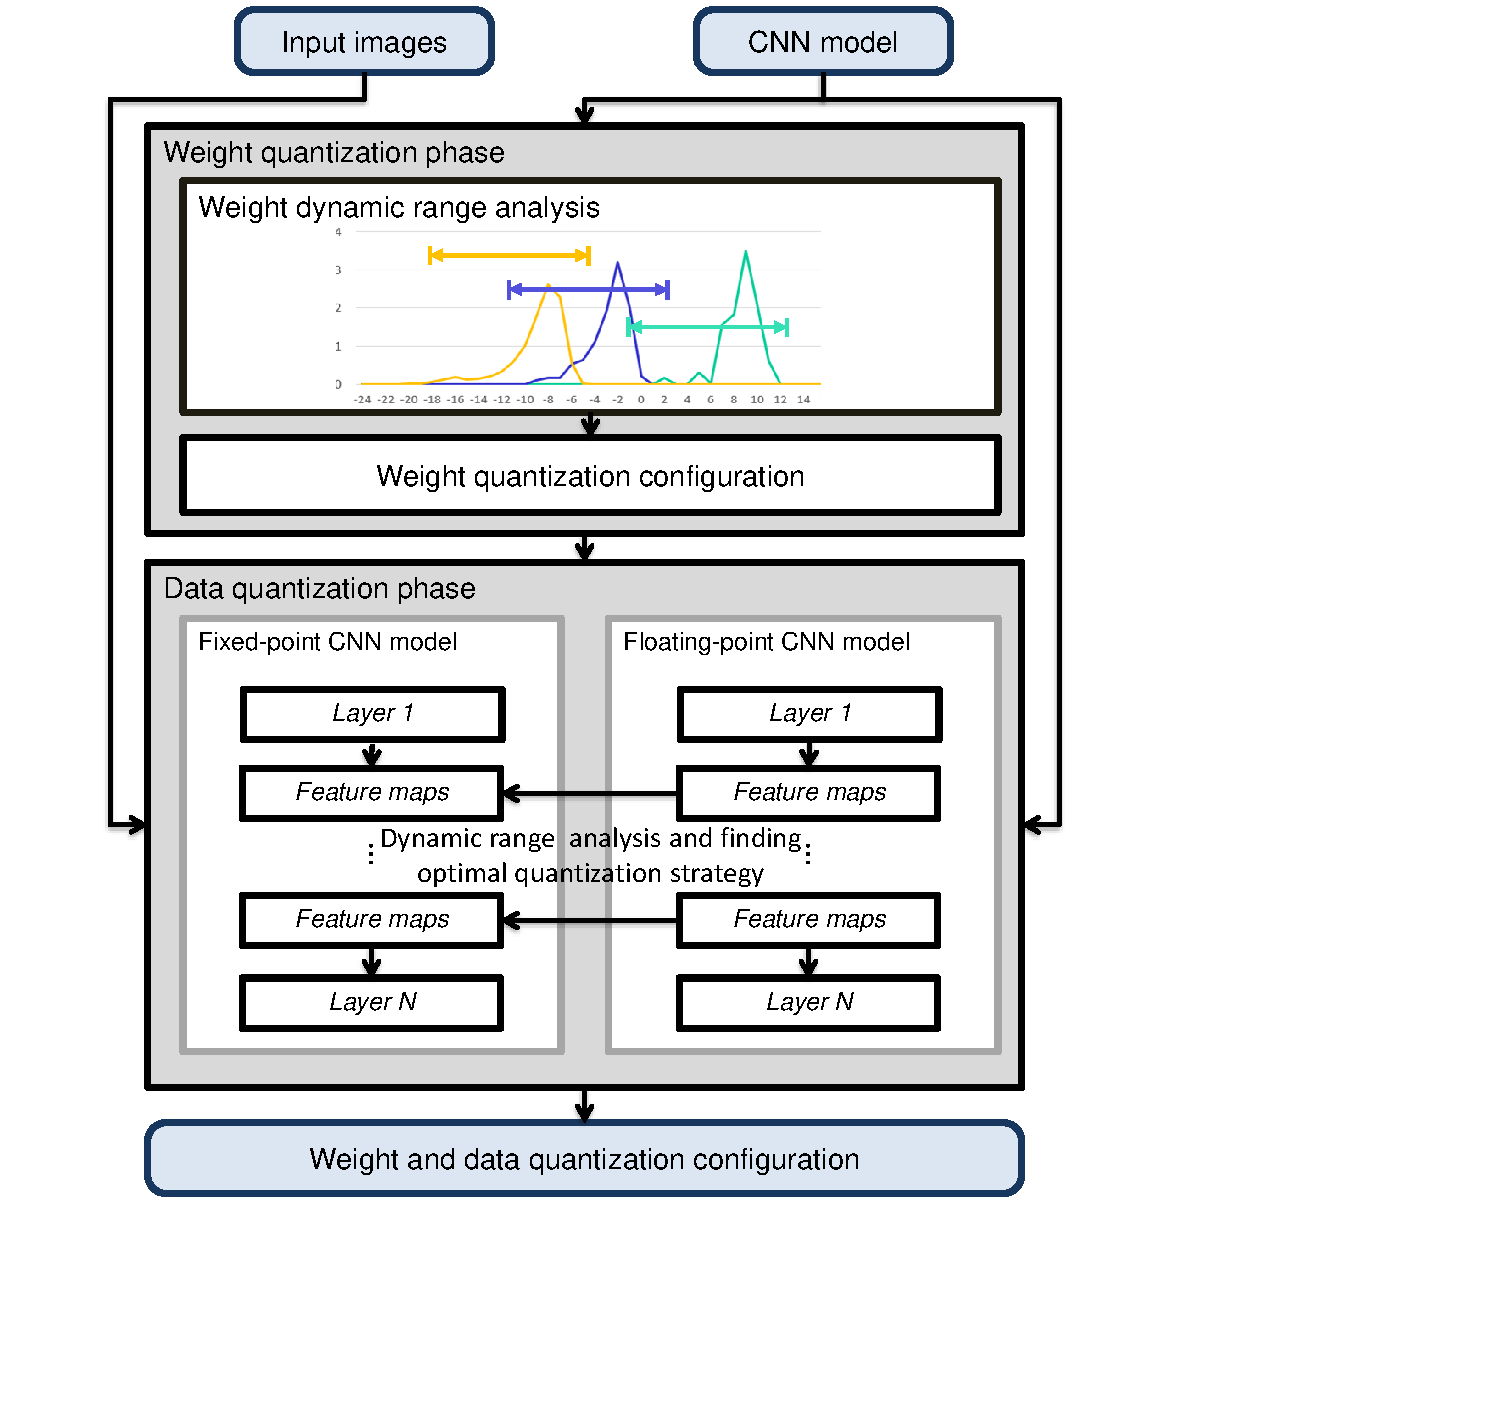
\includegraphics[width=1.0\columnwidth]{figure/quantization_flow.eps}
    \small
    %\vspace{-18pt}
    \caption{Data quantization flow~\cite{qiu2016going}}
    %\vspace{-10pt}
    \label{fig:quantization}
\end{figure}


\subsection{Hardware Architecture}
The proposed hardware architecture is shown in Figure~\ref{fig:arch}. It can be divided into four parts: PE array, On-chip Buffer, External Memory and Controller. Compared with our previous work~\cite{qiu2016going}, we isolate the core logic from a host ARM core and add some features to make a more general design.

\begin{figure}[t]
    \centering
    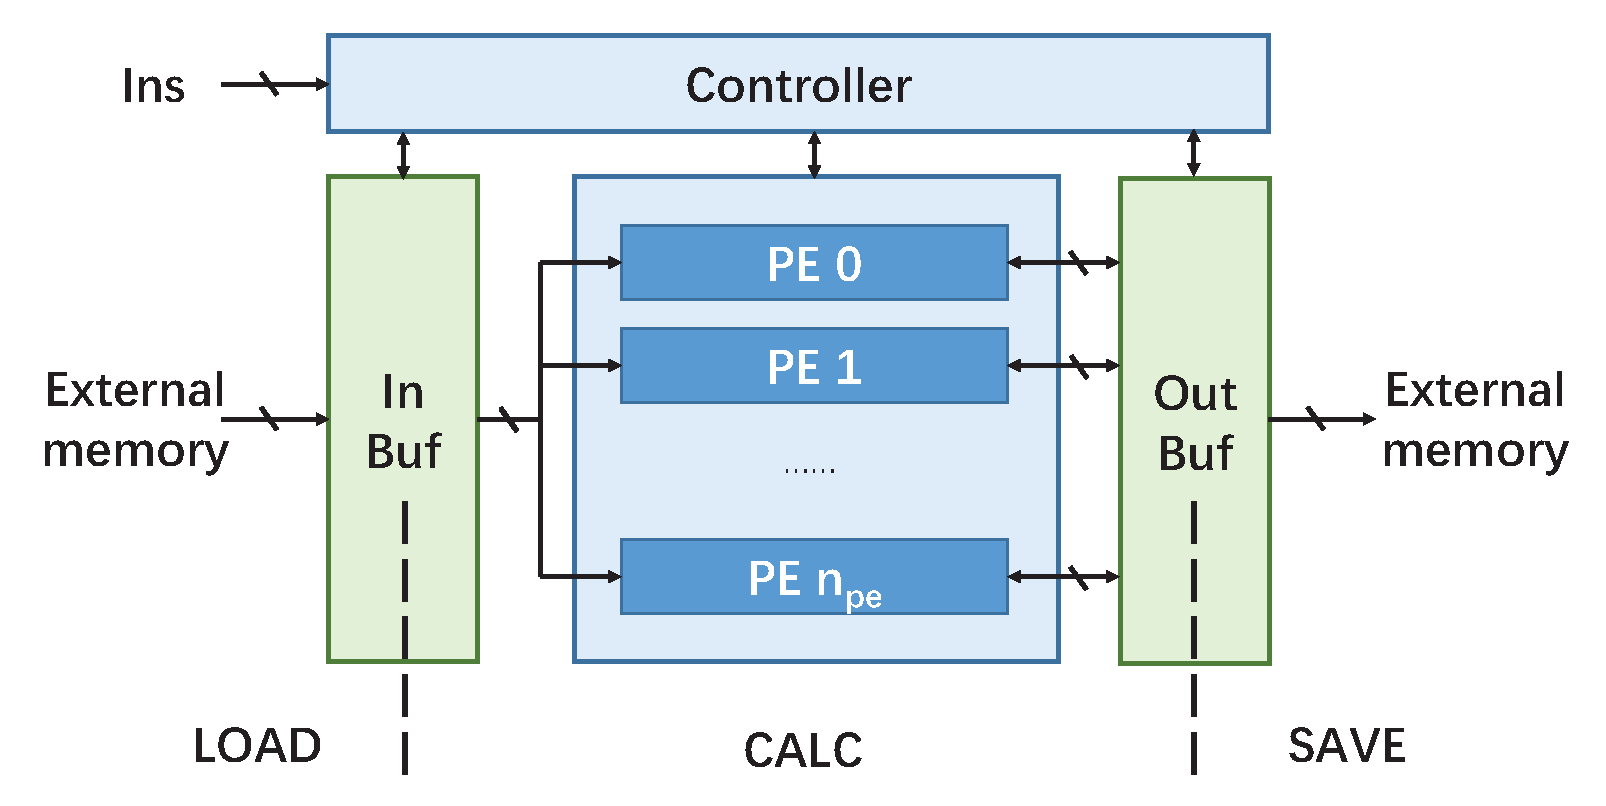
\includegraphics[width=1.0\columnwidth]{figure/hw_arch.eps}
    \small
    %\vspace{-10pt}
    \caption{Overall architecture of Angel-Eye}
    %\vspace{-5pt}
    \label{fig:arch}
\end{figure}

\textbf{PE Array}: Two levels of parallelism are implemented by PE array: inter-PE and intra-PE. Different PEs share the same input channels and use different kernels to calculate different output channels in parallel. Detailed structure of a single PE is shown in Figure~\ref{fig:pe}. Within each PE, different convolvers calculate 2D convolution on different input channels in parallel. The convolvers employ the line buffer design~\cite{bosi1999reconfigurable} and achieve kernel level parallelization. A 3$\times$3 kernel design is adopted because this size is most commonly used in state-of-the-art CNNs. It also supports kernels of smaller size by padding and kernels of larger size by time division multiplexing. The number of PE and convolvers are parameterized to fit into different platforms.

\begin{figure}[t]
  \centering
  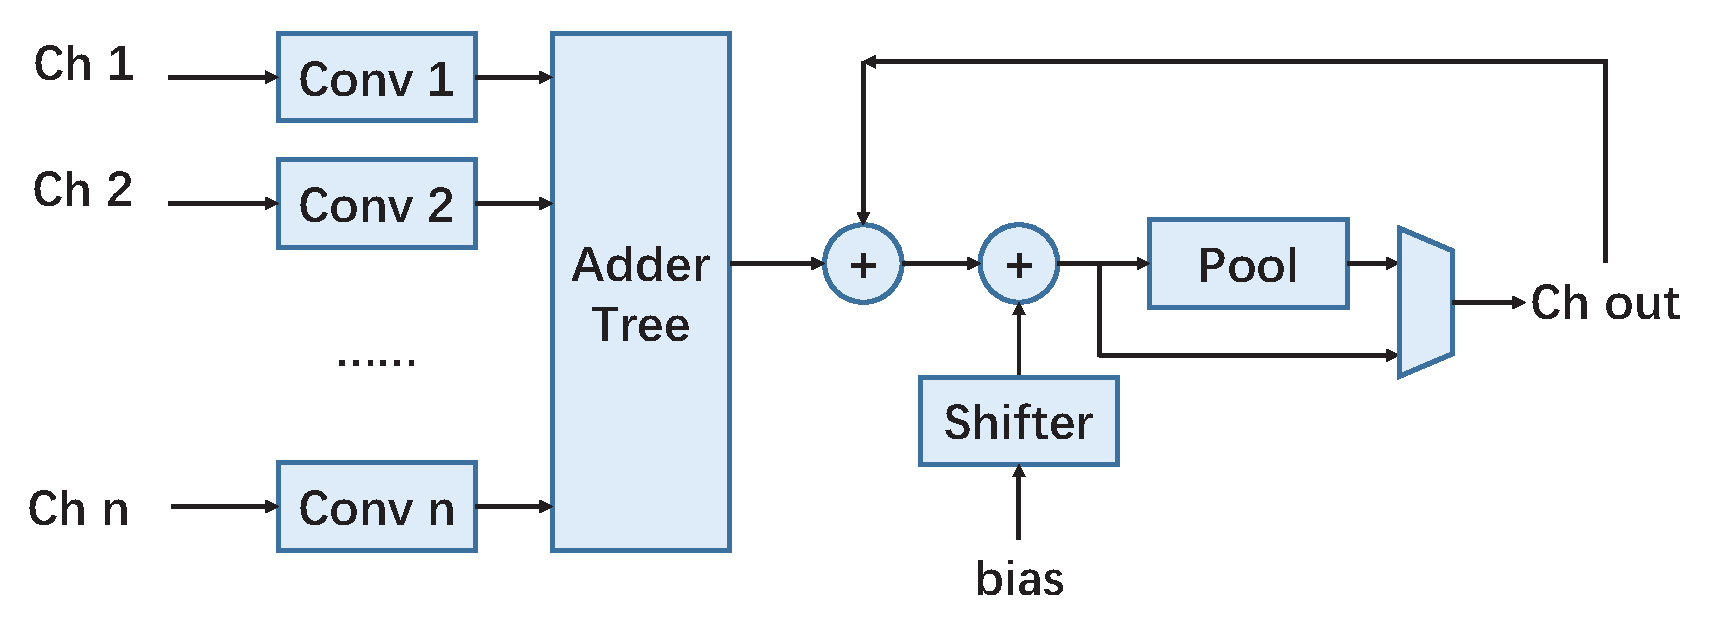
\includegraphics[width=1.0\columnwidth]{figure/pe.eps}
  \small
  %\vspace{-10pt}
  \caption{Structure of a single PE}
  %\vspace{-10pt}
  \label{fig:pe}
\end{figure}

\textbf{On-chip Buffer} This part separates PE Array with External Memory. This means data I/O and calculation can be parallelized. Output buffer also offers intermediate result to PE Array if more than one round of calculation is needed for an output channel. We introduce a 2-D description interface to manage the data. This enables the user to fully utilize the on-chip buffer. For example, a ping-pong strategy can be implemented by manually split the address space for ping and pong. For small layers, all the input channels can be loaded on chip. This reduce redundant external memory access.

\textbf{External Memory} For state-of-the-art CNN, On-chip Buffer is usually insufficient to cache all the parameters and data. External memory is used to save all the parameters of the network and the result of each layer.

\textbf{Controller} This part receives, decodes and issues instructions to the other three parts. Controller monitors the work state of each part and checks if the current instruction can be issued. Thus the host can send the generated instructions to Controller through a simple FIFO interface and wait for the work to finish by checking the state registers in Controller.  Figure~\ref{fig:controller} shows the structure of this part. The data dependency problem will be discussed in section~\ref{sec:ins_comp}.

\begin{figure}[t]
    \centering
    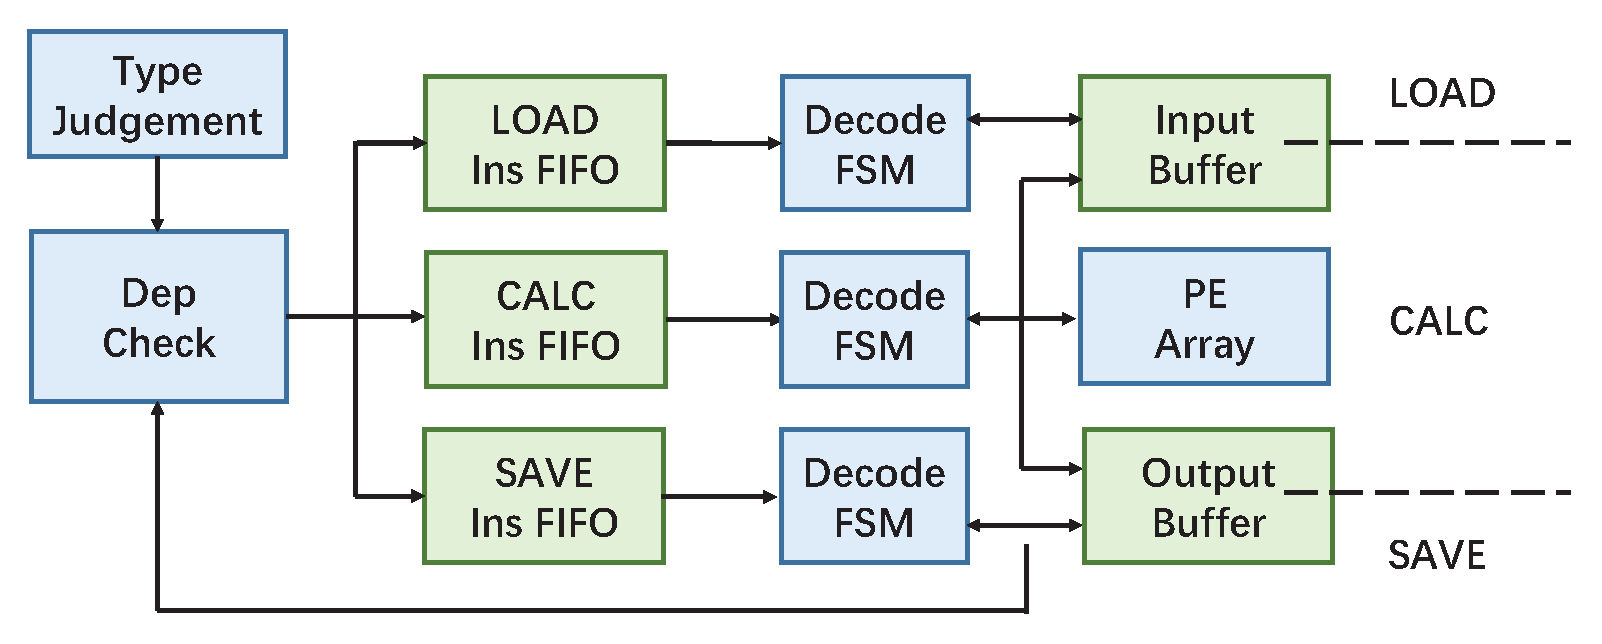
\includegraphics[width=1.0\columnwidth]{figure/controller.eps}
    \small
    %\vspace{-10pt}
    \caption{Structure of Controller}
    %\vspace{-5pt}
    \label{fig:controller}
\end{figure}

\subsection{Instruction Set and Compiler} \label{sec:ins_comp}
For this CNN accelerator, an instruction set of three instructions: LOAD, SAVE, and CALC, is proposed, corresponding to the I/O with external memory and the calculation done by PE Array. Address and size parameters for data in External Memory and On-chip Buffer are all embedded in instructions. Padding, pooling and data shift options can be set in CALC instructions. In this case, the hardware can support different networks by simply changing software.

Although I/O with external memory can be parallelized with calculation, there is latent data dependency problem. We set three flag bits in each instruction denoting if this instruction depends on the last previous LOAD or CALC or SAVE instruction. The schedule strategy can thus be managed during compilation and no extra workload is needed for the host at runtime.

A compiler is proposed to map a network descriptor file to hardware instructions. For each layer, the compiler tries to optimize the calculation time first. If various choices exist, it tries to minimize external memory access to reduce the power and bandwidth cost. The compiler is parameterized to support different hardware designs.

\begin{table*}[t]
    \centering
    \caption{Hardware Parameter and Resource utilization}
    \label{tab:resource}
    %\vspace{-5pt}
    \scriptsize
    \begin{tabular}{|c|c|c|c|c|c|c|c|c|} \hline
        design & data & \#PE & \#Conv & FF & LUT & BRAM & DSP & Clock\\ \hline
        XC7Z045 & 16-bit & 2 & 64 & 127653(29\%) & 182616(84\%) & 486(89\%) & 780(87\%) & 150MHz\\ \hline
        XC7Z020 & 8-bit & 2 & 16 & 24184(23\%) & 27215(51\%) & 68(49\%) & 198(90\%) & 100MHz \\ \hline
    \end{tabular}
    %\vspace{-5pt}
\end{table*}

\section{Experiment}\label{sec:experiment}
In this section, the proposed data quantization strategy is analyzed on different state-of-the-art CNNs. The hardware peformance is then evaluated with the quantized networks.

\subsection{Data Quantization Result}
The proposed data quantization strategy is evaluated on four networks: CaffeNet, which is a replication of AlexNet, VGG network, GoogLeNet~\cite{szegedy2014going}, and SqueezeNet.
50 images are used to optimize the radix position of each layer. 5000 images are used to test the classification accuracy of the network. Experimental results are shown in Table~\ref{tab:quantization}.

\begin{figure}[t]
  \centering
  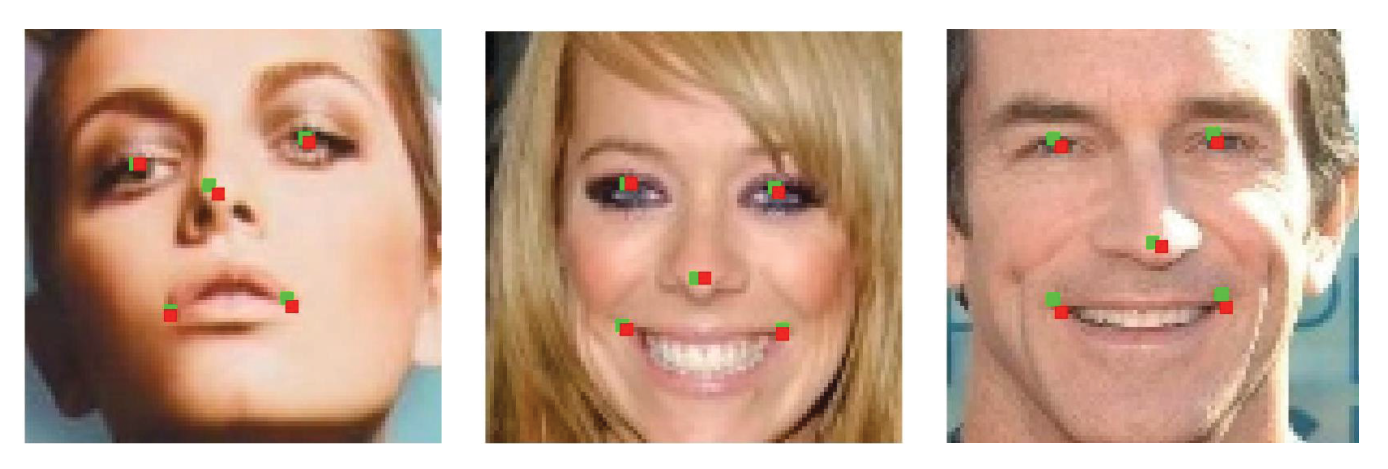
\includegraphics[width=1.0\columnwidth]{figure/alignment_result.eps}
  \small
  \vspace{-10pt}
  \caption{Five point face alignment result. Red points: floating-point network result. Green points: 8-bit fixed point network result.}
  \vspace{-10pt}
  \label{fig:face_align_res}
\end{figure}
For CaffeNet, the top 5 hit rate decreases about $1\%$ by 8-bit fixed point quantization. For VGG network, 16-bit fixed point compression introduce only $0.06\%$ extra top-5 error rate. That for the 8-bit form is $0.62\%$, which is negligible in common cases. For GoogLeNet and SqueezeNet, less than $1\%$ accuracy loss is brought by 8-bit quantization.

We also tested this strategy on the face alignment network in Figure~\ref{fig:face_align_net}. Compared with classification, this task requires a higher data precision. Example alignment results are shown in Figure~\ref{fig:face_align_res}. The coordinate error is within 2 pixels.

\begin{table}[ht]
\centering
    \begin{threeparttable}
        \caption{Exploration of different data quantization strategies with state-of-the-art CNNs.}
        \label{tab:quantization}
%        \setlength{\tabcolsep}{5pt}
%        \linespread{1.2}
        \begin{tabular}{|c|c|c|c|c|}
        \hline
        \multirow{2}[2]{*}{Network} & Data  & Weight & Top1  & Top5 \\
              & bitwidth & bitwidth & Accuracy & Accuracy \\
        \hline
        \multirow{3}[6]{*}{CaffeNet} & \multicolumn{2}{c|}{float} & 53.90\% & 77.70\% \\
    \cline{2-5}          & 16    & 16    & 53.90\% & 77.12\% \\
    \cline{2-5}          & 8     & 8     & 53.02\% & 76.64\% \\
        \hline
        \multirow{3}[6]{*}{VGG16} & \multicolumn{2}{c|}{float} & 68.10\% & 88.10\% \\
    \cline{2-5}          & 8     & 16    & 66.58\% & 87.38\% \\
    \cline{2-5}          & 8     & 8 or 4 & 66.96\% & 87.60\% \\
        \hline
        \multirow{4}[8]{*}{GoogLeNet} & \multicolumn{2}{c|}{float} & 68.62\% & 88.82\% \\
    \cline{2-5}          & 16    & 16    & 68.60\% & 88.82\% \\
    \cline{2-5}          & 8     & 8     & 68.40\% & 88.64\% \\
    \cline{2-5}          & 6     & 6     & 65.14\% & 86.50\% \\
        \hline
        \multirow{4}[8]{*}{SqueezeNet} & \multicolumn{2}{c|}{float} & 57.02\% & 79.72\% \\
    \cline{2-5}          & 16    & 16    & 57.04\% & 79.72\% \\
    \cline{2-5}          & 8     & 8     & 55.82\% & 79.16\% \\
    \cline{2-5}          & 6     & 6     & 39.28\% & 63.86\% \\
        \hline
        \end{tabular}

        \begin{tablenotes}
            \item[1] The weight bits "8 or 4" means 8 bits for CONV layers and 4 bits for FC layers.
        \end{tablenotes}
    \end{threeparttable}
\end{table}



\subsection{Hardware Performance}
Two FPGA based design of the hardware architecture is carried out. A 16-bit version of the design is implemented on the Xilinx XC7Z045 chip which targets at high performance applications. An 8-bit version is implemented on the Xilinx XC7Z020 chip which targets at low power applications.

The hardware parameter and resource utilization of our design is shown in Table \ref{tab:resource}. By choosing the design parameters properly, we can fully utilize the on-chip resource. Note that we are not using all the resource on XC7Z020 because the design coexists with an HDMI display logic for our demo. The clock speed is also affected by the routing difficulty on XC7Z020 where the resource is quite limited.

For the implementation on XC7Z045, we test it with VGG-16 network. The result together with that of similar work is shown in Table~\ref{tab:perf7045}. It can be seen that the proposed system gives out the best energy efficiency. Only the convolution layers are considered in this experiment though FC layer is also supported.

\begin{table}[t]
    \centering
    \begin{threeparttable}
        \caption{Performance comparison of Angel-Eye on XC7Z045 with other FPGA designs\cite{qiu2016going}}
        \label{tab:perf7045}
        %\vspace{-5pt}
        \scriptsize
        \begin{tabular}{|c|c|c|c|c|} \hline
            & {\bf\cite{chakradhar2010dynamically}}
            & {\bf\cite{gokhale2014240} }
            & {\bf\cite{zhang2015optimizing} }
            & {\bf Angel-Eye} \\ \hline
            \multirow
                {2}{*}{{\bf Platform}} & Virtex5 & Zynq & Virtex7 & Zynq \\
                                       & SX240t  & XC7Z045 & VX485t  & XC7Z045 \\ \hline
            {\bf Clock($\bf MHz$)} & 120 & 150 & 100  & 150 \\ \hline
            {\bf Bandwidth (GB/s)} & --  & 4.2 & 12.8 & 4.2 \\ \hline
            {\bf Quantization} & \multirow{2}{*}{48-bit fixed} & \multirow{2}{*}{16-bit fixed}  & \multirow{2}{*}{32-bit float} & \multirow{2}{*}{16-bit fixed} \\ {\bf Strategy} & & & & \\ \hline
            {\bf Power ($\bf W$)} & 14 & 8 & 18.61 & 9.63 \\ \hline
            {\bf Performance}  & \multirow{2}{*}{16} & \multirow{2}{*}{$23.18^1$} & \multirow{2}{*}{61.62} & \multirow{2}{*}{187.80} \\
            {\bf (GOP/s)} & & & & \\ \hline
            {\bf Energy Efficiency} & \multirow{2}{*}{1.14} & \multirow{2}{*}{2.90} & \multirow{2}{*}{3.31} & \multirow{2}{*}{19.50} \\ {\bf (GOP/J)}  & & & & \\ \hline
        \end{tabular}

        \begin{tablenotes}
            \item[1] The performance is of the face detector application in \cite{gokhale2014240} where the 552M-op network is running at 42 frames per second.
        \end{tablenotes}
    %\vspace{-10pt}
    \end{threeparttable}
\end{table}

For the implementation on XC7Z020, a face detection task is used to test the whole system. Face proposals are first generated by traditional CV algorithm. The CNN shown in Figure~\ref{fig:face_align_net} is then run on FPGA to do alignment. We aggressively compress the model to 8-bit fixed point for this task and the test result is quite accurate. A demo video is available at: https://youtu.be/m4e1SV89Dpg. The performance comparison with NVIDIA Terga K1 is shown in Table~\ref{tab:perf7020}. Angel-Eye on XC7Z020 is 7$\times$ and 2.6$\times$ faster and is also 20$\times$ and 15$\times$ more energy efficient.
\begin{table}[t]
    \centering
    \caption{Performance comparison of Angel-Eye on XC7Z202 with TK1 on 5-point face alignment task}
    \label{tab:perf7020}
    %\vspace{-5pt}
    \scriptsize
    \begin{tabular}{|c|c|c|c|} \hline
        & CPU(TK1) & GPU(TK1) & Angel-Eye(XC7Z020) \\ \hline
        \bf{Performance} & \multirow{2}{*}{2.73} & \multirow{2}{*}{7.31} &
        \multirow{2}{*}{19.2} \\
        \bf{(GOP/s)} & & & \\ \hline
        \bf{Speed(ms/f)} & 38.3 & 14.3 & 5.45 \\ \hline
        \bf{Power(W)} & \multicolumn{2}{c|}{5-10} & 2 \\ \hline
    \end{tabular}
    %\vspace{-10pt}
\end{table}

\section{Conclusion}\label{sec:conclusion}
In this paper, we propose a complete flow for mapping CNN onto customized hardware. This includes network quantization, flexible hardware architecture, and a compiler bridges the gap between them. Experimental results show that the generated design leads both in speed and energy efficiency compared with peer FPGA designs or implementations on mobile GPU. Future work will focus on better network compression strategy with corresponding hardware.

\section*{Acknowledgment}
Yu Wang's work was supported by 973 project 2013CB329000, National Natural Science Foundation of China (No. 61373026, 61261160501), the Importation and Development of High-Caliber Talents Project of Beijing Municipal Institutions, Microsoft, Xilinx University Program, and Tsinghua University Initiative Scientific Research Program.


\small
\bibliographystyle{IEEEtran}
\bibliography{ref}


\end{document}
